\chapter{Methods}

I developed a simulation model with three variants, based on the model presented by Chisholm \textit{et al.,} (2016). The variants consist of the Classic Model, and two modifications (Depth Model and Perimeter Model) for use in microbial TARs. I verified the simulation data by comparison to analytic results from the simplified equation presented by Chisholm \textit{et al.,} (2016) (2.2). The model fitting procedure was validated by fitting the model to simulation data with known parameters. The model fitting procedure was then applied to empirical data from the literature.  

\section{The Model}
\noindent The model describes a metacommunity and an island community. The metacommunity represents a source population from which propagules can immigrate to an island. Both communities are made up of \textit{K} non-overlapping niches. We assume that area is measured in number of individuals present ($\rho$ = 1). Neutral theory assumes that an individual's probability of birth and death do not depend on its species or density. In my model, each niche follows two suppositions of ecological neutral theory: niches operate under a zero-sum assumption (where community size is constant) and each species within the niche is considered ecologically equivalent (with the same probability of producing a propagule or dying). The metacommunity is generated by a modified coalescence algorithm \cite{rosindell2008coalescence} (see Supplementary Materials, Figure 7.1). A separate metacommunity is generated for each of \textit{K} niches and each niche consists of 10 000 individuals (\textit{J}). The metacommunity is assumed to be constant over timescales relevant to the island communities.\\

\noindent Each island niche is initiated with one unique species. At each timestep I process one randomly selected niche of every island. One individual in that niche dies and leaves a gap for another individual of a species suitable to occupy that niche. With probability \textit{m} (the per capita immigration rate), the dead individual is replaced with a randomly chosen propagule from the metacommunity. Species may only immigrate from the same niche in the metacommunity, to the corresponding niche in the island community. With probability 1 - \textit{m}, the dead individual is replaced with a local propagule from the same niche. The species richness for each island is stored every 5000 timesteps.\\

 \begin{figure}[h!]
\centering
  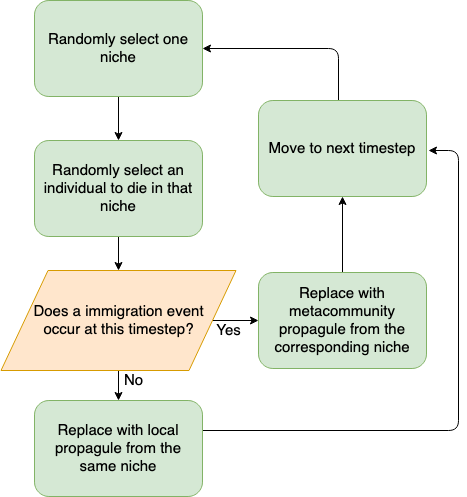
\includegraphics[scale=0.5]{SimFlow.png}
  \caption{Flowchart of simulation design}
  \label{fig:Flowchart}
\end{figure}

\noindent The probability of an immigration event occurring at each birth/death event (\textit{m}) is calculated with three variations, the Classic Model, the Depth Model and Perimeter Model (Figure 2.2). \textit{m\textsubscript{0}} is the immigration constant parameter from which \textit{m} is calculated. The Classic Model is the original model presented by Chisholm \textit{et al} (2016) and is most appropriate for species utilising aerial or directed dispersal, where immigration rate is directly proportional to area. The Depth Model simulates immigration into a three-dimensional space where species inhabit depth as well as area. For the Depth Model, each island simulation is given a depth of 1 unit. The Perimeter Model calculates \textit{m} as proportional to perimeter, for species that immigrate across land or water and whose likelihood of encountering a habitat is based on its perimeter. \\


 \begin{figure}[h!]
\centering
  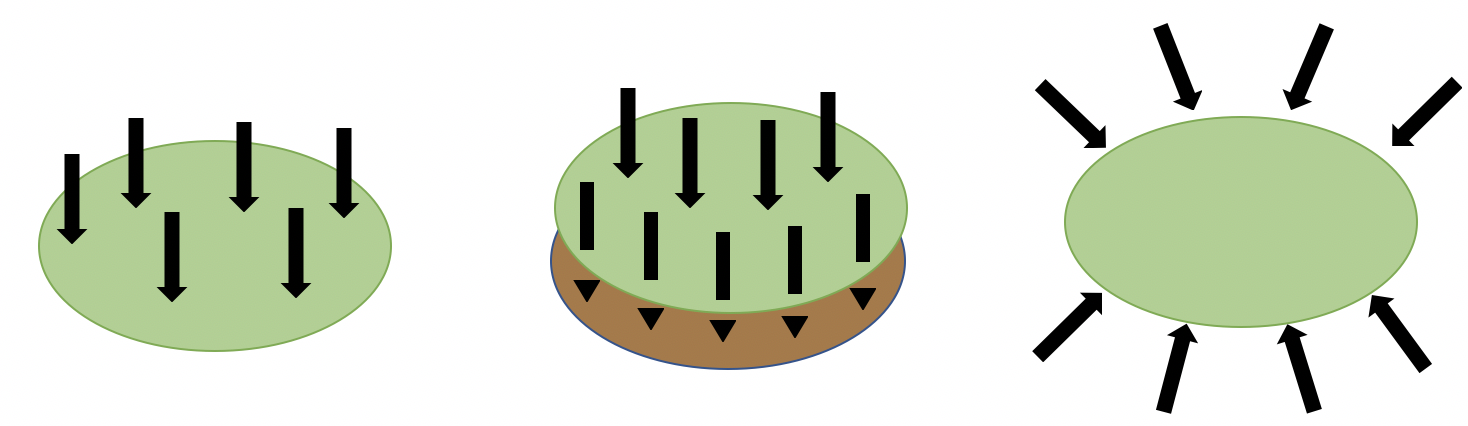
\includegraphics[scale=0.5]{models.png}
  \caption{\textbf{Classic} (\textit{m=m\textsubscript{0}}), \textbf{Depth} (\textit{m=m\textsubscript{0}/depth}), \textbf{Perimeter} (\textit{m=m\textsubscript{0}/$\protect\sqrt{area}$}) }
  \label{fig:Models}
\end{figure}

\noindent 


\noindent I ran 200 simulations 100 times for each of the three models (Classic, Depth and Perimeter) using the High Performance Computing (HPC) service at Imperial College London. The 200 simulations consisted of 20 island areas differing in powers of 2 multiplied by 10 unique parameter combinations (Table 2.1). \textit{m\textsubscript{0}} values for the Perimeter Model simulation were higher than those for the Classic and Depth Models, to allow the simulation to reach equilibrium within 24 hours. Parameter values are not indicative of real-world speciation or immigration rates and are arbitrary values to facilitated running the simulation to equilibrium within 24 hours. I plotted a timeseries for each simulation to ensure equilibrium has been reached, before calculating the mean species richness for each set of  simulation parameters.\\

\begin{table}[h]
\centering
    \caption{Simulation parameters where the same range of parameters is applied to each of the Classic, Depth and Perimeter Model simulations. Higher \textit{m\textsubscript{0}} values were given to the Perimeter Model simulation to allow it to reach equilibrium within 24 hours. Simulations with larger areas and low immigration rates (\textit{m}) take longer to reach equilibrium and for the Perimeter Model simulation \textit{m=m\textsubscript{0}/$\protect\sqrt{area}$} thus immigration rates were considerably lower than for the Classic and Depth Models}
    \label{crouch}
    \begin{tabular}{  l  p{5cm}}
        \toprule
\textbf{Parameter} 
&\textbf{Values}   \\\midrule
speciation rate (\textit{nu})
&0.00001 - 0.0001 \\\hline
immigration constant (\textit{m\textsubscript{0}})
&0.01 - 0.1 (0.09-0.1 Perimeter)\\\hline
number of niches (\textit{K})
&5 - 50 \\\hline
simulation areas (i.e. number of individuals)
& 5 - 20,000 \\
        \bottomrule
    \end{tabular}
\end{table}

 
\subsection{Validation and Model Fitting Procedure}

\noindent The results of the model were found analytically by applying the simplified mathematical model presented by Chisholm \textit{et al.,} (2.2-2.5).
Analytic and simulation results were compared to ensure the model had been simulated successfully. In these analytical solutions the species richness (\textit{S}) is given by: 

\begin{equation}
S=\theta\{\psi(\frac{\theta}{K}+\gamma(\psi(\gamma+J)-\psi(\gamma)))-\psi(\frac{\theta}{K})\}
\end{equation} 

\begin{center}
\noindent Where $\psi$ is the digamma function, \textit{J} is the number of individuals per niche, \textit{K} is the number of niches and $\theta$ is the fundamental biodiversity number calculated as \textit{nu*(J*K-1)/(1-nu)} 
\end{center}

\begin{equation}
\gamma=(J-1)m/(1-m)
\end{equation}

\begin{center}
and 
\end{center}

\begin{equation}
 m=m\textsubscript{0}
 \quad\mathrm{or}\quad
 m=m\textsubscript{0}/D   
 \quad\mathrm{or}\quad
 m = m\textsubscript{0}/\sqrt{A}
\end{equation}

\noindent Where \textit{m\textsubscript{0}} is the immigration constant used to calculate per capita immigration rate \textit{m}, \textit{D} = depth, \textit{A} = area and

\begin{equation}
J=A\;{\rho}/K
 \quad\mathrm{or}\quad
J=A\;{\rho}\;D/K
\end{equation}

\noindent Where \textit{J = A\;$\rho$/K} is used for the two-dimensional models (Classic and Perimeter) and \textit{J = A\;$\rho$\;D/K} is used for the three-dimensional model (Depth). For all simulations $\rho$ is given as 1 as area (\textit{A}) is measured in units corresponding to number of individuals. \\

\noindent The mathematical model was fit to the simulation data using non-linear least squares (NLLS) fitting in R (version 3.6.1 (2019-07-05)). The model fitting procedure uses the minpack.lm package. This package provides a Levenberg-Marquardt NLLS fitting function (nlsLM) that uses a more robust algorithm than it's base-R counterpart. \\

{\texorpdfstring

\noindent \noindent  The three fitted parameters of the model are \textit{K}, \textit{m\textsubscript{0}} and $\theta$. To aid the fitting procedure values of \textit{K} were looped through from 1 to maximum species richness and from this \textit{\^{m\textsubscript{0}}} and $\hat{\theta}$ starting values were calculated, where A\textsubscript{med} is median surface area of habitats, S\textsubscript{A\textsubscript{max}} is species richness in the largest habitat and W\textsubscript{-1}(\textit{x}) is the lower branch of the Lambert W function. The best-fit values were stored for the \textit{K} and corresponding \textit{m\textsubscript{0}} and ${\theta}$ that gave the highest R\textsuperscript{2} score. They were calculated as follows:

\begin{equation}
\hat{m\textsubscript{0}}=\frac{-K}{{\rho}\;A_{med}\;W_{-1}\;(-K\;{\rho}\;A_{med})}
\end{equation}

\begin{equation}
\hat{\theta}=\frac{S_{A_{max}}\;\hat{\gamma}\;log\;\hat{m\textsubscript{0}}}{S_{A_{max}}-\hat{\gamma}\;log\;\hat{m\textsubscript{0}}\;W_{-1}(exp(S_{A_{max}}/\hat{\gamma}\;log\hat{m\textsubscript{0}}\;S_{A_{max}})/(\hat{\gamma}\;log\;\hat{m\textsubscript{0}}))}
\end{equation} \\

\begin{center}
Where $\hat{\gamma}$ is calculated as:\\
\end{center}

\begin{equation}
\hat{\gamma}=\frac{({\rho}\;A_{max})-1)\hat{m\textsubscript{0}}}{1-\hat{m\textsubscript{0}}}
\end{equation}\\

\noindent Using NLLS to fit the three models to their corresponding simulations I was able to validate the fitting procedure by recapturing the known parameters (\textit{K}, \textit{m\textsubscript{0}} and $\theta$).


\subsection{Critical Area}


\noindent The critical area of transition from niche-structured regime to extinction-colonisation equilibrium regime (\textit{A\textsubscript{crit}}) where the TAR starts to increase to a steeper gradient can be calculated as:

\begin{center}
\textbf{Classic Model}
\end{center}

\begin{equation}
A\textsubscript{crit}=\frac{\theta(1-m\textsubscript{0})(exp(K/\theta)-1)}{m\textsubscript{0}\;\rho\;log(1/m)} 
\end{equation}\\

\begin{center}
\textbf{Depth Model}
\end{center}

\begin{equation}
A\textsubscript{crit}=\frac{1}{\rho\; D}\left[\frac{{\theta}(exp^\frac{K}{\theta}-1)(D - m\textsubscript{0})}{m\textsubscript{0}\;log(\frac{m\textsubscript{0}}{D})}+1\right]
\end{equation}\\

\begin{center}
\textbf{Perimeter Model}
\end{center}

\begin{equation}
x = \frac{\theta(exp^\frac{K}{\theta}-1)}{m\textsubscript{0}{\rho}}
 \quad\mathrm{and}\quad
A\textsubscript{crit}=\left\{\frac{x}{W_{0}(x/m\textsubscript{0})}\right\}^2
\end{equation}\\

\noindent For each model fitting, \textit{A\textsubscript{crit}} is estimated from the best-fit parameters of \textit{K}, $\theta$ and \textit{m\textsubscript{0}}. For higher values of \textit{K} and lower values of $\theta$, \textit{m\textsubscript{0}} and $\rho$, \textit{A\textsubscript{crit}} will be larger.  \textit{A\textsubscript{crit}} formulas were validated by visual inspection of fits to the simulation data. \\

\noindent With parameter estimations obtained from the NLLS fitting of the three models to empirical datasets, \textit{A\textsubscript{crit}} was estimated. For habitats with varying area and depth values \textit{A\textsubscript{crit}} was calculated for each depth value, the mean taken then multiplied by the mean depth of the dataset to give a mean critical volume (\textit{V\textsubscript{crit}}) and plotted with habitat volume (depth x area) and species richness. The mean \textit{A\textsubscript{crit}} from these fittings is used in the statistical analysis for comparison with homogenous depth habitats. By finding \textit{A\textsubscript{crit}} for empirical datasets, I was able to test the theory that regime shift would occur at lower areas for less isolated habitats and for more motile taxa.


\section{Data Collection and Analysis}

\begin{table}[h!]
  \begin{center}
    \caption{Summary of datasets collected from the literature}
    \label{table2}
    \pgfplotstabletypeset[
      multicolumn names, % allows to have multicolumn names
      col sep=comma, % the seperator in our .csv file
      display columns/0/.style={
		column name=$Taxa$, % name of first column
		string type},  % use siunitx for formatting
      display columns/1/.style={
		column name=$Habitat$, % name of first column
		string type},  % use siunitx for formatting
      display columns/2/.style={
		column name=$Count$,
		column type={S},string type},
           every head row/.style={
		before row={\toprule}, % have a rule at top
		after row={
			%\si{\ampere} & \si{\volt}\\ % the units seperated by &
			\midrule} % rule under units
			},
		every last row/.style={after row=\bottomrule}, % rule at bottom
    ]{SummaryTab.csv} % filename/path to file
  \end{center}
\end{table}

\noindent I compiled 57 datasets from 29 studies on microbial TARs (Table 2.2) (see Supplementary Materials, Table 7.1). They include a range of taxonomic groups and habitat types. Before model fitting, datasets without positive correlation between area and OTU richness were excluded. Datasets with a positive correlation were imported into each of the three NLLS fitting scripts (Classic, Depth, Perimeter). $\rho$ was estimated separately from the other three parameters. Estimations were taken from the original study or proxy papers (see Supplementary Material, Table 7.2). I also fitted each dataset with the simple power-law model (Introduction, Equation 1.1) and the model fit is compared to each of the Classic, Depth and Perimeter models using Akaike Information Criterion (AIC) score to determine if, by incorporating $\theta$, \textit{K}, \textit{m\textsubscript{0}} and $\rho$ parameters, our models are better fits to the data. \\ 

\section{Statistical Analysis}

{\texorpdfstring
Foor empirical datasets where adjusted R\textsuperscript{2} was between 0 and 1 and at least one of the three models was a reasonable fit, I found the mean R\textsuperscript{2} and adjusted R\textsuperscript{2} as well as the standard deviation and range. For datasets that were equally well fit to two or more of the models I found the mean \textit{A\textsubscript{crit}} and parameter estimations ($\theta$, \textit{m\textsubscript{0}}, \textit{K}) for each of those fittings and used these in the analysis. The median, standard deviation and range of the fitted parameters was found and correlation tests carried out. Differences between mean \textit{A\textsubscript{crit}} across habitat types and taxonomic groups was found. Multiple regression analysis of log \textit{A\textsubscript{crit}} was carried out with habitat type and taxonomic group as categorical explanatory variables. }



